% !TeX root = ../main.tex

\chapter{石墨烯的其他性质与应用、市场前景}

\section{石墨烯的光学性质}

参考图~\ref{fig:grapheneDiracPoint},对于本征石墨烯,其费米能点位于狄拉克点处,此时电子可以通过带间跃迁的方式从价带跃迁到能带。特别的,针对\textit{n}型或是\textit{p}型掺杂的石墨烯,费米能级会发生移动,以\textit{n}型掺杂为例,掺入的电子将填充导带底,致使费米能级上移,此时导带底部和价带顶部的电子吸收一定能量后都可发生跃迁。在如此特殊的能带结构下,石墨烯有着其他半导体材料所不具有的特殊的光学性质。

\subsection{线性光学性质}

由于石墨烯独特的电子能带结构,本征单层石墨烯的动力学光导与入射光频率无关,可用以下公式表示:

\begin{equation}
    G_1(\omega) = G_0 \equiv e^2/4\hbar
\end{equation}

其中,$\omega$为入射光频率,$e$为电子电荷,$\hbar$为普朗克常数。

本征石墨烯的光学透过率在宽光谱敢为内只取决于其精细结构常数$\alpha = e^2/\hbar c$($c$为光速),可用以下公式表示:

\begin{equation}
    T \equiv (1+2\pi G/c)^{-2} \approx 1-\pi \alpha
\end{equation}

另外,石墨烯带内光电导率和带间光导率均与化学式和入射光频率相关。值得注意的是,带内光电导率$\sigma_{intra}$与石墨烯的等离子增强效应和和表面等离基元传输密切相关。

\subsection{非线性光学性质}

当入射光所在电场与石墨烯内碳原子的外层电子发生共振时,石墨烯内电子云相对于原子核的位置发生偏移,产生极化,最终导致了石墨烯的非线性光学性质。

在外加光场的强度较弱时,产生的极化强度与外加电场$E$呈现线性依赖的关系,可用以下公式表示:

\begin{equation}
    P = \epsilon_0 x^{(1)}E
\end{equation}

其中$\epsilon_0$为真空介电常数,$x^{(1)}$为一阶线性极化率。

在外加光场的强度很强,电子云偏移较大的时候,电子极化强度$P$与$X$、$E$呈现非线性依赖关系:

\begin{equation}
    P = \epsilon_0 x^{(2)}E^2 + \epsilon_0 x^{(3)}E^3 + \ldots \epsilon_0 x^{(n)}E^n +\ldots
\end{equation}

其中$x^{(2)}$和$x^{(3)}$分别为二阶非线性极化率和三阶非线性极化率,均与石墨烯的饱和吸收特性、光学双稳态等非线性光学特性相关。

对于一节线性极化率$x^{(1)}$,实部代表了石墨烯折射率,虚部代表了光学增益或光学损耗。通过改变施加垂直表面的直流电场,可以有效调节$x^{(1)}$的数值,进而改变石墨烯的折射率。由于反演对称性,$x^{(2)}$通常认为为$0$。石墨烯的三阶非线性极化率$x^{(3)}$与石墨烯的许多非线性光学性质相关,如饱和吸收、自聚焦、克尔效应、光学双稳态以及孤波传播等。

\section{光学性质的应用}

光学性质的应用主要集中在以下方面:

\begin{itemize}
    \item 锁模光纤激光器
    \item 调 Q 光纤激光器
    \item 固体激光器
    \item 直波导结构光调制器
    \item 垂直透射式结构光调制器
    \item 超快、宽波段光探测器
    \item 共振腔增强的光探测器
    \item 波导型光探测器
    \item 叠层范德华异质结型光探测器
    \item 基于石墨烯等离子体的太赫兹激光器和天线
          % \item 发光二极管
\end{itemize}

\section{石墨烯的其他性质}
石墨烯片具有超高的力学强度,这是由于极强的碳-碳键相互作用。石墨烯的杨氏模量有$1TPa$\cite{RN43},断裂强度达$130GPa$,断裂强度超过普通钢材强度的$200$多倍\cite{RN43},是目前力学强度最高的材料。

石墨烯也具有优秀的导热性。在室温条件下其热导率为$(5.3±0.48)×103 W/m \cdot K$,最高可达到$6000 W/m \cdot K$\cite{RN44},明显高于纳米级碳纳米管的导热率$(3500  W/m \cdot K)$。石墨烯也是目前热导率最好的材料。
石墨烯的表面积大,且透明。单层石墨烯片的表面积为$2630m^{2}$g。且经过红外光谱的分析发现单层石墨烯仅有少量的光吸收,透光率达$97.7\%$ \cite{RN45,RN46},几乎完全透明。
化学性质上,由于碳-碳键组成的石墨烯在性质上与苯环相似,然而石墨烯是由多个六元环组成导致了许多性质又有所不同。从宏观上看,石墨是由许多多层的石墨烯叠加而成,使得石墨烯同时具有稠环的部分性质和石墨的化学性质。


\section{石墨烯的其他性质的应用}
\subsection{石墨烯新型吸附剂}
石墨烯、氧化石墨烯以其层絮状结构、优异特性及其功能化改性等特征可作为新型吸附剂材料,在环境水体和土壤中污染的修复、大气污染治理等方面具有较大的应用潜力。例如石墨烯/碳(G/C)复合气凝胶可以吸附水中污染物土霉素、布洛芬;\cite{lee2008measurement}聚合离子液体修饰的氧化石墨烯吸附剂能够用于工业废水等水体中去除亚甲基蓝的新型吸附剂\cite{lilulu}。

\subsection{石墨烯储氢}
石墨烯储氢即石墨烯虽然可以隔绝所有气体和液体,却能够对质子“网开一面”。科学家设计出的“三明治结构”将碳氮材料夹在两层石墨烯中,然后再利用光能产生激子,这些光能产生的激子分离后会形成正负电荷,并分别分布于外层石墨烯和碳氮“夹心”层。

石墨烯表面的水分子在正电荷的帮助下分解,产生质子。这些质子可穿透石墨烯,并在遇到电子后发生反应,进而产生氢气。由于只有质子能够通过石墨烯,而产生的氢气不能穿透石墨烯,所以光解水产生的氢气分子会被安全地保留在“三明治结构”内。同时氧原子、氧气、羟基等物质无法进入复合体系,从而抑制了氧与氢重新变为水的逆反应发生,实现了高储氢率下的安全储氢。

石墨烯对氢气的极强的吸附能力可以引入到氢能源汽车及飞机等交通工具领域,将带来良好的经济、环境、社会效益。

\subsection{氧化石墨烯抑菌性及应用}
氧化石墨烯(GO)是含氧官能团分布在表面及边缘上,并伴有部分缺陷位点的单层石墨烯。2010年上海应用物理所樊春海课题组以GO为抗菌剂,对革兰氏阴性大肠杆菌的杀菌效果进行研究,结果表明,浓度为$85\mu g/mL$的GO经过2h的接触时间后能够几乎完全抑制大肠杆菌的生长,抑菌率达$98.5\%$。\cite{pannengyu}

目前关于GO抗菌性能有三种主流机理,分别为来自GO纳米级锋利的边缘的膜穿刺,活性氧(ROS)依赖或非依赖引起的氧化应激作用,以及GO柔性薄膜结构对细菌的缠绕或捕获。

利用GO的抑菌性,可以明显抑制大肠杆菌的滋生,龋病、牙周炎及种植体周围炎主要致病菌如链球菌、牙龈卟啉单胞菌、具核梭杆菌等,这对人体细胞是无害的。

\section{市场前景}

自石墨烯成功制备以来,其在科学界造成了巨大反响。石墨烯是一种低维材料,具有优良的导电性、光电子特性、特殊的量子隧穿效应、超导特性、理论上存在的量子反常霍尔效应,以及特殊的力学、热学与化学性质。随着其制备方式的不断改进和工业化发展,这些性质逐步得到工业上的广泛应用,并逐渐展现出广阔的市场前景,一点一滴地改变着我们的生活。

石墨烯材料一经发现,由于其性质的特殊性立刻收到了广泛的关注。诺奖得主海姆曾表示:“一般来说,一个新材料从实验室走到产业化需要40年左右的时间,但是石墨烯只用了不到10年。”其新兴材料的市场化进程速度之快出乎所有人意料,究其原因,一方面是其性质的广泛应用性(已在前文叙述过),另一方面是其制备方法的不断完善和进步。

石墨烯刚刚被发现时,价格为500元/g,现如今为1000元/kg,这充分说明了随着制备技术进步,石墨烯制备原料易得化、工艺简明化,工艺制造成本已出现大幅下降(这在中科大无机化学实验课本中收录制备石墨烯作为教学实验中可见一斑);成本下降意味着市场准入门槛下降,而在我国这个投资、消费和出口都十分丰富的市场,石墨烯产业正呈一派欣欣向荣之势:产值上,我国2020年石墨烯总产能约1万吨,且根据天眼查数据,截至2021年11月30日,我国已注册石墨烯企业11432家;在应用广度、创新性上,同样可圈可点,根据中国石墨烯联盟(CGIA)秘书长李义春在第八届中国国际石墨烯创新大会所表示的,目前国内石墨烯专利申请量累计达6.9万件,专利申请量占全球78.18\%。2020年市场规模为140亿元,2025年市场规模预计达到1000亿元。

\begin{figure}
    \centering
    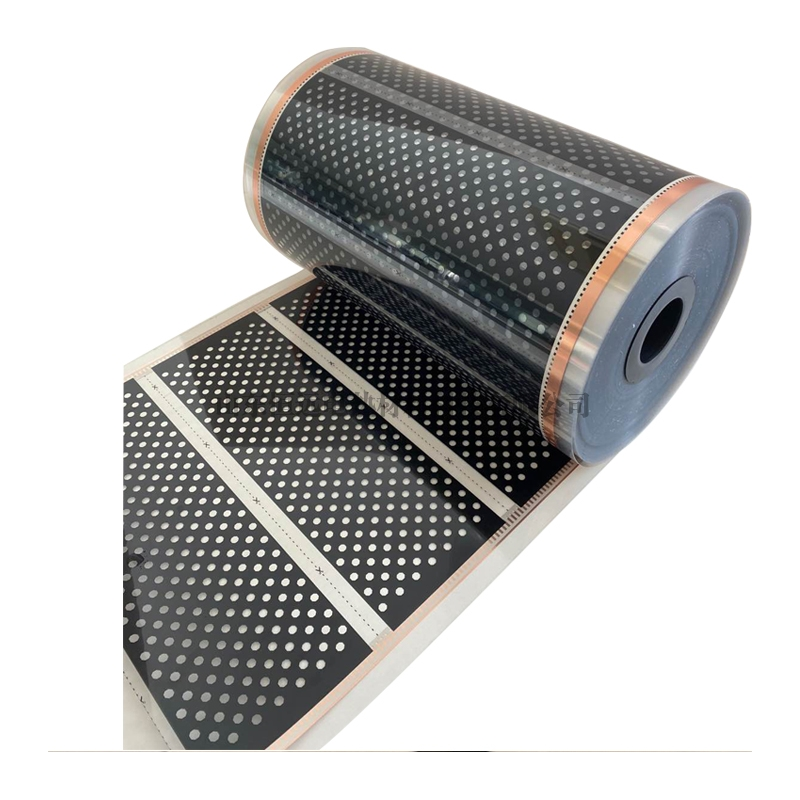
\includegraphics[scale=0.2]{img/6.png}
    \caption{石墨烯地暖}
\end{figure}

但是,繁华背后,石墨烯的市场竞争力存在很大的问题。石墨烯存在严重的产能利用率\footnote{工业总产出对生产设备的比率,就是实际生产能力到底有多少在运转发挥生产作用}不足的问题。石墨烯产能利用率较之其他工业很低,2020年四个季度的全国工业产能利用率依次为67.3\%,74.4\%,76.7\%,78.0\%\footnote{数据来源:国家统计局官网},但石墨烯产业2020年全年产能利用率不足5\%。“材料学如何发论文?往材料里掺石墨烯”已沦为坊间笑柄,虽然与事实差距很大,但一阵见血地指出了石墨烯创新性的虚假繁荣:只是凭借性质的独特,对从口罩到地暖形形色色商品的特质进行了“不定向”的改变,且不会发生质变,在市场中大部分并不能发挥不可替代的作用,不具备“核心竞争力”;这给该产业带来了硬伤。

\begin{figure}
    \centering
    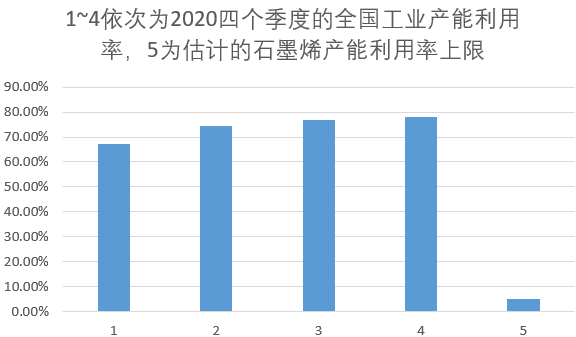
\includegraphics[scale=0.6]{img/7.png}
    % \caption{图为MATTG的TBKT-D-ν三维图,其中D为电位移,$ν=4n/n_s$}
\end{figure}

石墨烯在发现之初是打算替代硅作为应用于芯片领域的,为何难以实现呢?由于石墨烯基本没有带隙,当前技术是无法切断其永久性导电性的。倘若随着技术进步,这一难题被克服,石墨烯这一材料在市场依然是大有前程的。

尽管现如今石墨烯在市场存在很多问题,它依然是一种很优秀的材料:除了因技术和成本限制其并未推广的很多具有不可替代性的应用,其更重要的价值在于其奇特的性质,为前沿的科学理论提供实验依据或实验验证;科学是对未来的投资,比起商家在石墨烯相关商品买卖中赚取的蝇头小利,也许石墨烯在科研人员实验室中、论文上才能体现自己真正的价值。

\chapter{结束语}
自石墨烯成功制备以来,其在科学界造成了巨大反响。石墨烯是一种低维材料,具有优良的导电性、特殊的量子隧穿效应、超导特性、量子霍尔效应,以及特殊的力学、热学、光学与化学性质。随着其制备方式的不断改进和工业化发展,这些性质逐步得到工业上的广泛应用,并逐渐展现出广阔的市场前景,一点一滴地改变着我们的生活。